\documentclass[polish,aspectratio=169]{beamer}

% wide screen
% \documentclass[aspectratio=169]{beamer}


%%% YOUR PACKAGES HERE %%%
\usepackage{comment}
\usepackage{hyperref}
\usepackage[backend=biber, style=numeric, bibstyle=ieee,
            sorting=none, isbn=false, urldate=ymd,
            doi=false, url=true]{biblatex}
\addbibresource{bibliography/bibliography.bib}
\renewbibmacro{in:}{}
\usepackage{subfigure}
\usepackage{graphicx}
\usepackage{geometry}
\usepackage{float}
\usepackage{listings}
\usepackage{xcolor}

\newcommand{\refrys}[1]{Rys.~\ref{#1}}
\newcommand{\reflist}[1]{List.~\ref{#1}}
\newcommand{\refEq}[1]{Równ.~\ref{#1}}
% \usepackage{tikz} 
% \usetikzlibrary{graphs,graphs.standard,automata}


% polish language
\usepackage[polish]{babel}
\usepackage{polski}



%%% IMPORT PG PRESENTATION STYLE %%%
% THIS IS GDANSK UNIVERSITY OF TECHNLOGOGY (PG) PRESENTATION TEMPLATE
% Creator: Jan Cychnerski <jan.cychnerski@eti.pg.edu.pl>
% Copyleft 2019


% PG THEME OPTIONS

\usetheme{Boadilla}
\usecolortheme{default}
\usefonttheme{professionalfonts}

% colors

\definecolor{PGBlue}{RGB}{0,56,101}
\definecolor{PGRed}{RGB}{193,10,39}
\definecolor{PGSilver}{RGB}{200,200,200}
\definecolor{PGBlack}{RGB}{0,0,0}

% PGBlue
\setbeamercolor{frametitle}{fg=PGBlue}
\setbeamercolor{normal text}{fg=PGBlue}
\setbeamercolor{structure}{fg=PGBlue}
\setbeamercolor{item}{fg=PGBlue}

% PGRed
\setbeamercolor{alerted text}{fg=PGRed}
\setbeamercolor{item projected}{fg=PGRed}

% white
\setbeamercolor{title}{fg=white}
\setbeamercolor{titlelike}{fg=white}
\setbeamercolor{subtitle}{fg=white}

% enumerate and itemize styles

\setbeamertemplate{itemize item}{\bfseries\color{PGRed}\raise1pt\hbox{\donotcoloroutermaths$\bullet$}}
\setbeamertemplate{itemize subitem}{\color{PGRed}\raise0.5pt\hbox{--}}
\setbeamertemplate{itemize subsubitem}{\color{PGRed}\tiny\raise1.5pt\hbox{\donotcoloroutermaths$\bullet$}}

\setbeamertemplate{enumerate item}{\bfseries\color{PGRed}\insertenumlabel.}
\setbeamertemplate{enumerate subitem}{\color{PGRed}\insertsubenumlabel.}
\setbeamertemplate{enumerate subsubitem}{\color{PGRed}\insertsubsubenumlabel.}
\setbeamertemplate{enumerate mini template}{\insertenumlabel}


% disable navigation

\beamertemplatenavigationsymbolsempty

% additional commands

\newcommand*{\vcenteredhbox}[1]{\begingroup
\setbox0=\hbox{#1}\parbox{\wd0}{\box0}\endgroup}

\graphicspath{{pgbeamer/}}


\usepackage{iflang}
\IfLanguageName{polish}{
\newcommand{\pglogobig}{pg-logo-big-pl}
\newcommand{\pglogosmall}{pg-logo-small-pl}
}{
\newcommand{\pglogobig}{pg-logo-big-en}
\newcommand{\pglogosmall}{pg-logo-small-en}
}


% FRAME TITLE LOGO
\addtobeamertemplate{frametitle}{\vcenteredhbox{\includegraphics[height=8mm]{\pglogosmall}}\bfseries}{}


\newcommand{\pgtitleframe}{{
% PG TITLE PAGE

\setbeamercolor{background canvas}{bg=PGBlue}
\setbeamercolor{title}{fg=white}
\setbeamercolor*{date}{fg=white}
\setbeamercolor*{author}{fg=white}

\setbeamertemplate{footline}{}

\begin{frame}[noframenumbering]
\centering
\vspace{1cm}
\includegraphics[height=3cm]{\pglogobig}
\vspace{5mm}
\maketitle
\end{frame}
}}

\newcommand{\pglastframe}{{
% PG LAST PAGE

\setbeamercolor{background canvas}{bg=PGBlue}
\setbeamercolor{title}{fg=white}
\setbeamercolor*{date}{fg=white}
\setbeamercolor*{author}{fg=white}

\setbeamertemplate{footline}{}

\begin{frame}[noframenumbering]
\centering
\vspace{1cm}
\includegraphics[height=5cm]{\pglogobig}
\end{frame}
}}



%%% YOUR OPTIONS HERE %%%

\title[Jak wiele informacji o sobie udostępniamy w Internecie]{Jak wiele informacji o sobie udostępniamy w Internecie}
\subtitle{}
\author{Marek Borzyszkowski \and Paulina Brzęcka}
\date{\today}

\setbeamercovered{invisible}
\begin{document}

\pgtitleframe

\begin{frame}{Plan pracy}
  \begin{columns}[c]
    \column{.5\textwidth}
    \begin{enumerate}
      \item Analiza podstawowych danych i budowa profilu.
      \item Źródła pozyskiwania informacji.
      \item Wykorzystanie danych przez różne podmioty.
      \item Zagrożenia wynikające z udostępniania danych.
      \item Zalecenia dotyczące ochrony prywatności.
    \end{enumerate}
    \column{.5\textwidth}
    \begin{figure}
      \centering
      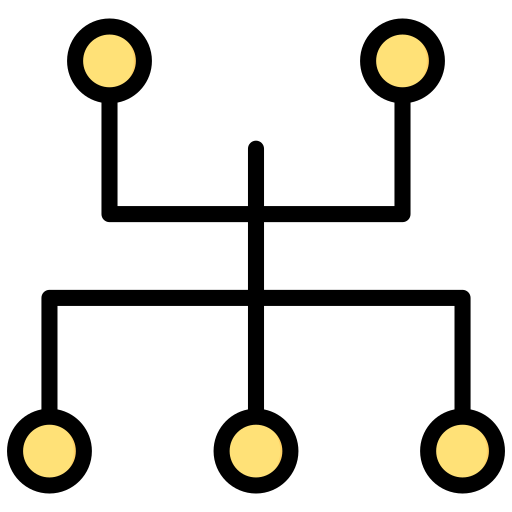
\includegraphics[height=0.45\textheight]{images/network-topology.png}
    \end{figure}
\end{columns}
\end{frame}

\begin{frame}{Co znaleźliśmy w Internecie na ten temat?}
  \begin{columns}[c]
    \column{.5\textwidth}
    \begin{itemize}
      \item Rodzaje danych, które są ujawniane w internecie,
      \item Główne źródła danych,
      \item Typowe zagrożenia,
      \item Przykłady rzeczywistych incydentów,
      \item Działania zabezpieczające dane,
      \item Dostępne narzędzia do sprawdzania naruszeń danych.
    \end{itemize}
    \column{.5\textwidth}
    \begin{figure}
      \centering
      
\includegraphics[height=0.45\textheight]{images/social-network.png}
    \end{figure}
\end{columns}
\end{frame}

\begin{frame}{Wprowadzenie - czym są dane osobowe?}
    \begin{alertblock}{Dlaczego dane osobowe są istotne?}
      \begin{itemize}
        \item Dane osobowe to informacje umożliwiające identyfikację osoby fizycznej. \cite{PII_USDE}
        \item W Internecie udostępniamy je świadomie i nieświadomie.
        \item Ich analiza pozwala tworzyć dokładne profile użytkowników.
      \end{itemize}
    \end{alertblock}
  \end{frame}
  
  
  \begin{frame}{Dane jawnie udostępniane}
  \begin{columns}[c]
      \column{.5\textwidth}
      \begin{alertblock}{Co użytkownicy podają sami?}
        \begin{itemize}
          \item Nazwa użytkownika, zdjęcie profilowe, data urodzenia, imię, nazwisko
          \item Posty, komentarze, aktywność na forach
          \item Informacje udostępniane podczas zakupów lub rejestracji - od imienia i nazwiska, po adres zamieszkania. \cite{CYB_DEF_NAJCZĘSTRZE_DANE}
        \end{itemize}
      \end{alertblock}
      \column{.5\textwidth}
      \begin{figure}
        \centering
        
\includegraphics[height=0.45\textheight]{images/social-media.png}
        \label{fig:social-media}
      \end{figure}
  \end{columns}
  \end{frame}
  
  
  \begin{frame}{Dane techniczne i ukryte}
  \begin{columns}[c]
      \column{.5\textwidth}
      \begin{figure}
        \centering
        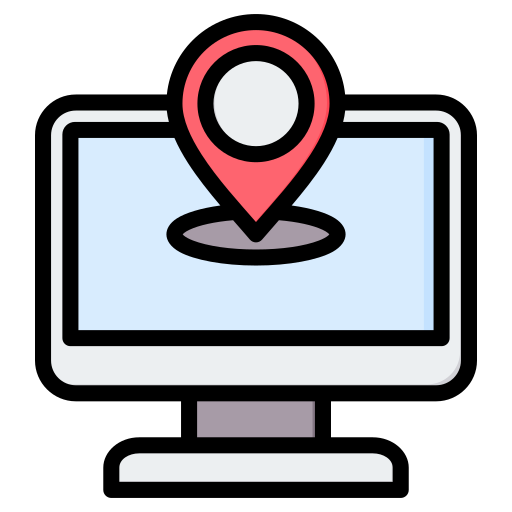
\includegraphics[height=0.45\textheight]{images/ip-address.png}
        \label{fig:ipTracking}
      \end{figure}
      \column{.5\textwidth}
      \begin{alertblock}{Co zbierane jest w tle?}
        \begin{itemize}
          \item Adres IP, nagłówki HTTP, czas trwania sesji
          \item Fingerprinting urządzenia - unikalna konfiguracja przeglądarki
          \item Pliki cookies i śledzenie międzystronowe
        \end{itemize}
      \end{alertblock}
  \end{columns}
  \end{frame}
  
  
  \begin{frame}{Dane jednoznacznie identyfikujące - wrażliwe}
    \begin{alertblock}{Informacje bezpośrednio wskazujące osobę}
      \begin{itemize}
        \item Numer PESEL, numer telefonu, adres e-mail
        \item Informacje z dokumentów tożsamości \cite{LEXDIGITAL_CZY_IMIE_NAZW_TO_DANE_OS}
      \end{itemize}
    \end{alertblock}
  \end{frame}
  
  
  \begin{frame}{Dane biometryczne i behawioralne}
    \begin{alertblock}{Jak zachowanie nas zdradza?}
      \begin{itemize}
        \item Głos, odciski palców, sposób chodzenia, rozpoznawanie twarzy
        \item Styl pisania, rytm korzystania z klawiatury/myszy
        \item Dane zbierane przez urządzenia i aplikacje mobilne
      \end{itemize}
    \end{alertblock}
  \end{frame}
  
  
  \begin{frame}{Case study: identyfikacja w badaniach DNA}
  \begin{columns}[c]
      \column{.5\textwidth}
      \begin{alertblock}{Czy dane genetyczne są naprawdę anonimowe?}
        \begin{itemize}
          \item Dane z publicznych baz (GEDmatch) wykorzystane do identyfikacji anonimowych uczestników badań DNA
          \item Połączenie danych genetycznych z metadanymi (wiek, miejsce) wystarczyło do identyfikacji 241 z 579 wybranych osób.\cite{DNA_LEAK}
        \end{itemize}
      \end{alertblock}
      \column{.5\textwidth}
      \begin{figure}
        \centering
        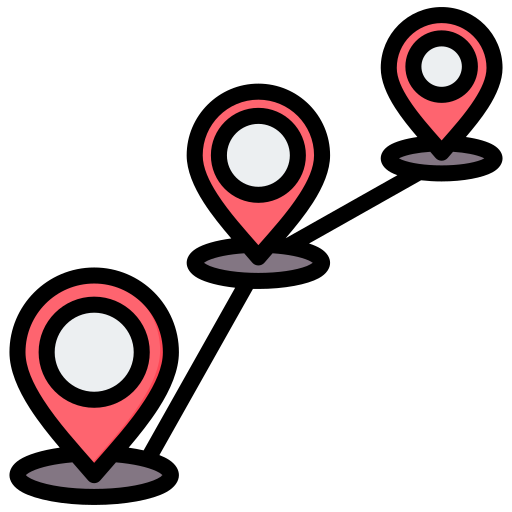
\includegraphics[height=0.45\textheight]{images/routing.png}
        \label{fig:dnaCase}
      \end{figure}
  \end{columns}
  \end{frame}
%--- Sekcja: Źródła publiczne ---
\section{Źródła publiczne danych}

\begin{frame}{Źródła publiczne - przegląd}
\begin{columns}[c]
    \column{.5\textwidth}
    \begin{alertblock}{Gdzie szukać danych?}
        \begin{itemize}
          \item Media społecznościowe \cite{zrodlo} \cite{zrodloArtykul}
          \item Fora, blogi, komentarze
          \item Rejestry publiczne \cite{zrodloDzialalnosc}
          \item Portale ogłoszeniowe, firmowe
          \item Urządzenia IoT \cite{zrodlo2}
          \item Narzędzia AI \cite{ai}
        \end{itemize}
        \end{alertblock}
    \column{.5\textwidth}
    \centering
    \begin{figure}
        \centering
        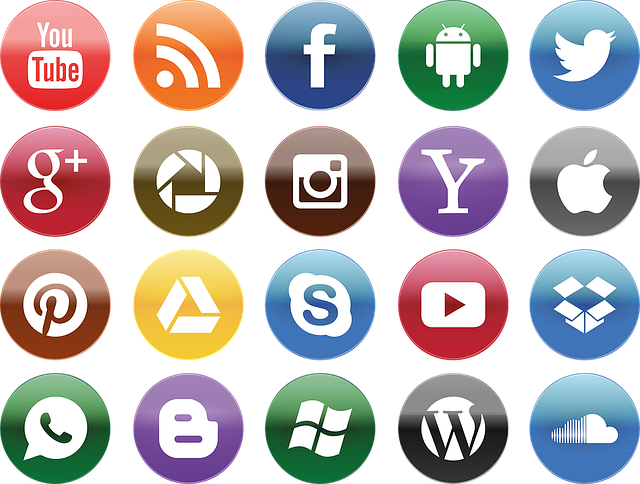
\includegraphics[width=0.75\textwidth]{images/socialMedia.png}
        \label{fig:socialMedia}
    \end{figure}    
\end{columns}
\end{frame}

% \begin{frame}{Media społecznościowe}
% \begin{block}{}
% \begin{itemize}
%   \item \textbf{Facebook}: dane osobowe, relacje, lokalizacje z postów
%   \item \textbf{X (Twitter)}: tweety, zdjęcia z geolokalizacją
%   \item \textbf{LinkedIn}: historia kariery, kontakty, sukcesy
%   \item \textbf{Blogi i fora}: styl pisania, emocje, IP, pseudonimy
%   \item \textbf{Ustawienia prywatności}: często ignorowane lub błędnie skonfigurowane \cite{zrodlo} \cite{zrodloArtykul}
% \end{itemize}
% \end{block}
% \end{frame}

% \begin{frame}{Rejestry i portale firmowe}
% \begin{block}{Ogólnodostępne bazy danych}
% \begin{itemize}
%   \item \textbf{CEIDG}: dane właścicieli firm jednoosobowych
%   \item \textbf{KRS}: członkowie zarządu, adresy siedzib
%   \item \textbf{CRBR}: beneficjenci rzeczywiści + numery PESEL udziałowców!
%   \item \textbf{E-Księgi Wieczyste}: właściciele nieruchomości
%   \item \textbf{Portale firmowe, ogłoszenia}: e-maile, telefony, nazwiska \cite{zrodloDzialalnosc}
% \end{itemize}
% \end{block}
% \end{frame}

% \begin{frame}{Urządzenia IoT}
% \begin{columns}[c]
%     \column{.5\textwidth}
%     \begin{itemize}
%         \item Monitorują obecność domowników
%         \item Ustalają rutyny, harmonogramy
%         \item Dane wykorzystywane marketingowo, czasem bez zgody!
%         \item Przykład: smart lodówka wie, co jesz i kiedy \cite{zrodlo2}
%       \end{itemize}
%     \column{.5\textwidth}
%     \centering
%     \begin{figure}
%         \centering
%         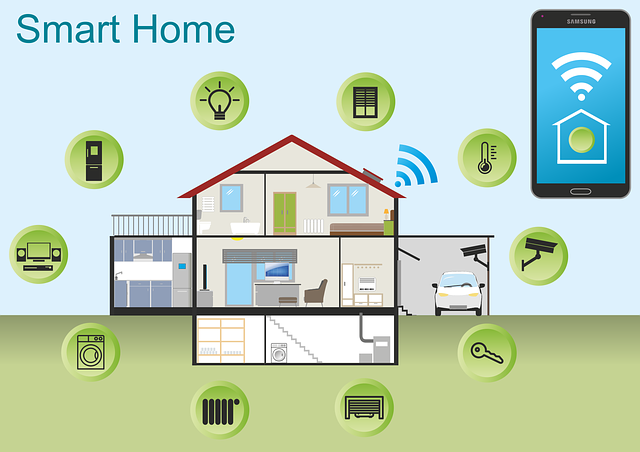
\includegraphics[width=1\textwidth]{images/smart-home.png}
%         \label{fig:smart-home}
%     \end{figure}    
% \end{columns}
% \end{frame}

% \begin{frame}{Czaty AI jako źródła danych}
% \begin{columns}[c]
%     \column{.5\textwidth}
%     \begin{block}{Zalety... i zagrożenia}
%         \begin{itemize}
%           \item 43\% pracowników korzysta z AI w pracy
%           \item Wiele firm nie kontroluje, co jest wpisywane
%           \item AI może zapamiętywać treści zapytań
%           \item Analiza stylu, kontekstu, tonu → profilowanie użytkowników \cite{ai}
%         \end{itemize}
%         \end{block}
%     \column{.5\textwidth}
%     \centering
%     \begin{figure}
%         \centering
%         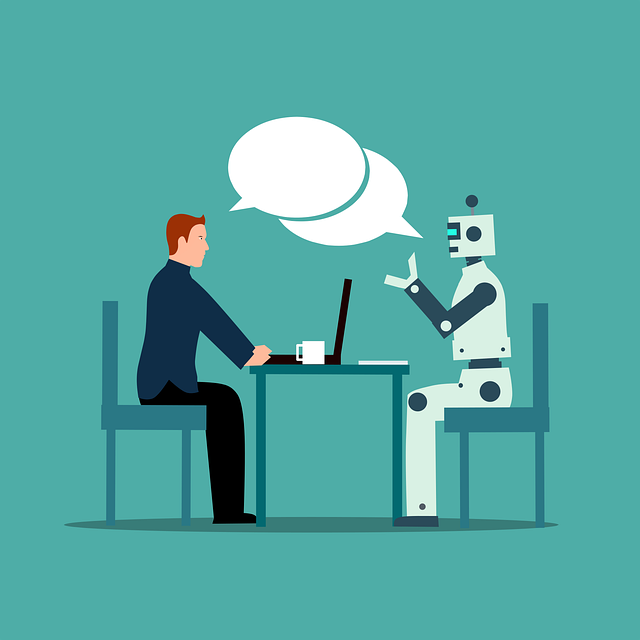
\includegraphics[width=0.75\textwidth]{images/interview.png}
%         \label{fig:interview}
%     \end{figure}    
% \end{columns}
% \end{frame}
    
    \begin{frame}{Dane jako zasób strategiczny}
    \begin{alertblock}{Dlaczego dane są cenne?}
        \begin{itemize}
          \item Dane to nowa forma kapitału - porównywalna z ropą czy złotem.
          % \item Pozwalają przewidywać zachowania i wpływać na decyzje.
          \item Są gromadzone masowo przez wiele podmiotów.
        \end{itemize}
    \end{alertblock}
    \end{frame}
    
    
    \begin{frame}{Firmy reklamowe i technologiczne}
    \begin{columns}[c]
        \column{.5\textwidth}
        \begin{alertblock}{Profilowanie i personalizacja}
            \begin{itemize}
              \item Dane z aktywności online służą do budowy profili.
              \item Użytkownik otrzymuje „spersonalizowaną rzeczywistość”.
              \item Reklamy, ceny, treści - wszystko dostosowane do profilu. \cite{EFF}
            \end{itemize}
        \end{alertblock}
        \column{.5\textwidth}
        \begin{figure}
          \centering
          
\includegraphics[height=0.45\textheight]{images/social-network.png}
        \end{figure}
    \end{columns}
    \end{frame}
    
    
    \begin{frame}{Pracodawcy i uczelnie}
    \begin{alertblock}{Decyzje oparte na danych}
        \begin{itemize}
          \item Dane z mediów społecznościowych mogą wpłynąć na decyzję o zatrudnieniu.\cite{DIGITAL_GLOBAL}
          \item Platformy e-learningowe śledzą aktywność studentów.
          % \item Uczelnie analizują zaangażowanie, postępy, a nawet emocje.
        \end{itemize}
    \end{alertblock}
    \end{frame}
    
    
    \begin{frame}{Instytucje państwowe i służby}
    \begin{columns}[c]
        \column{.5\textwidth}
        \begin{figure}
          \centering
          
\includegraphics[height=0.45\textheight]{images/user-management.png}
        \end{figure}
        \column{.5\textwidth}
        \begin{alertblock}{Zarządzanie i kontrola}
            \begin{itemize}
              \item Dane wykorzystywane są do nadzoru i przewidywania ryzyk.
              \item W Chinach działają systemy oceny obywateli.\cite{DIGITAL_LOCAL}
              \item W wielu krajach zbierane są dane z kamer, mediów i smartfonów.
            \end{itemize}
        \end{alertblock}
    \end{columns}
    \end{frame}
    
    
    \begin{frame}{Firmy ubezpieczeniowe i banki}
    \begin{alertblock}{Ryzyko obliczane danymi}
        \begin{itemize}
          \item Twoje nawyki zakupowe i lokalizacja wpływają na ocenę ryzyka.
          \item Styl jazdy może zwiększyć lub obniżyć składkę ubezpieczenia.
        \end{itemize}
    \end{alertblock}
    \end{frame}
    
    
    \begin{frame}{Cyberprzestępcy}
    \begin{columns}[c]
        \column{.5\textwidth}
        \begin{figure}
          \centering
          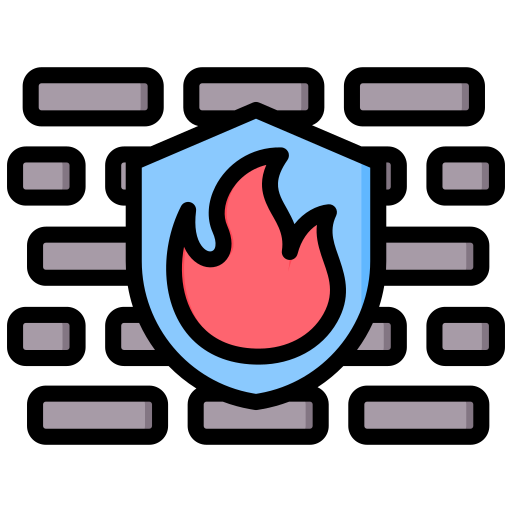
\includegraphics[height=0.45\textheight]{images/firewall.png}
        \end{figure}
        \column{.5\textwidth}
        \begin{alertblock}{Kto jeszcze się interesuje danymi?}
            \begin{itemize}
              \item Skradzione dane mogą zostać odsprzedane lub wykorzystane do szantażu.
              \item Phishing, kradzież tożsamości, podrabiane profile.\cite{PHISHING_REPORT}
              \item Często wykorzystywane są dane z przecieków publicznych.
            \end{itemize}
        \end{alertblock}
    \end{columns}
    \end{frame}
    
    \begin{frame}{Komu ufamy z naszymi danymi?}
    \begin{alertblock}{Zostawiamy więcej, niż nam się wydaje}
        \begin{itemize}
          % \item Nie wiemy, kto analizuje i przetwarza nasze dane.
          \item Coraz trudniej uniknąć śledzenia, nawet jeśli „nic nie udostępniamy”.
          \item Dane osobowe są paliwem cyfrowego świata - i zagrożeniem, i wartością.
        \end{itemize}
    \end{alertblock}
    \end{frame}
\section{Zagrożenia}
\begin{frame}{Zagrożenia}
    \begin{block}{Co może się wydarzyć?}
    \begin{itemize}
      \item Kradzież tożsamości
      \item Naruszenie prywatności i poufności danych
      \item Cyberstalking i nękanie
      \item Oszustwa socjotechniczne i internetowe
      \item Konsekwencje reputacyjne
      \item Odpowiedzialność prawna
    \end{itemize}
    \end{block}
\end{frame}

\begin{frame}{}
  \begin{center}
    {\huge Przykłady z życia}
  \end{center}
\end{frame}

\begin{frame}{Oferta sprzedaży bazy klientów Empiku}
\begin{columns}[c]
    \column{.5\textwidth}
    \begin{block}{}
      \begin{itemize}
        \item Marzec 2025
        \item Ogłoszenie dotyczące sprzedaży rzekomej bazy danych zawierającej informacje o 24 milionach klientów Empiku
        \item Baza miała zawierać takie dane jak: imię i nazwisko, numer telefonu, adresy i informacje o zamówieniach
      \end{itemize}
      \end{block}
    \begin{exampleblock}{Empik: reakcja}
    \begin{itemize}
      \item Szybka analiza
      \item Komunikacja z klientami
      \item Współpraca z zespołem CERT \cite{empik}
    \end{itemize}
    \end{exampleblock}
    \column{.5\textwidth}
    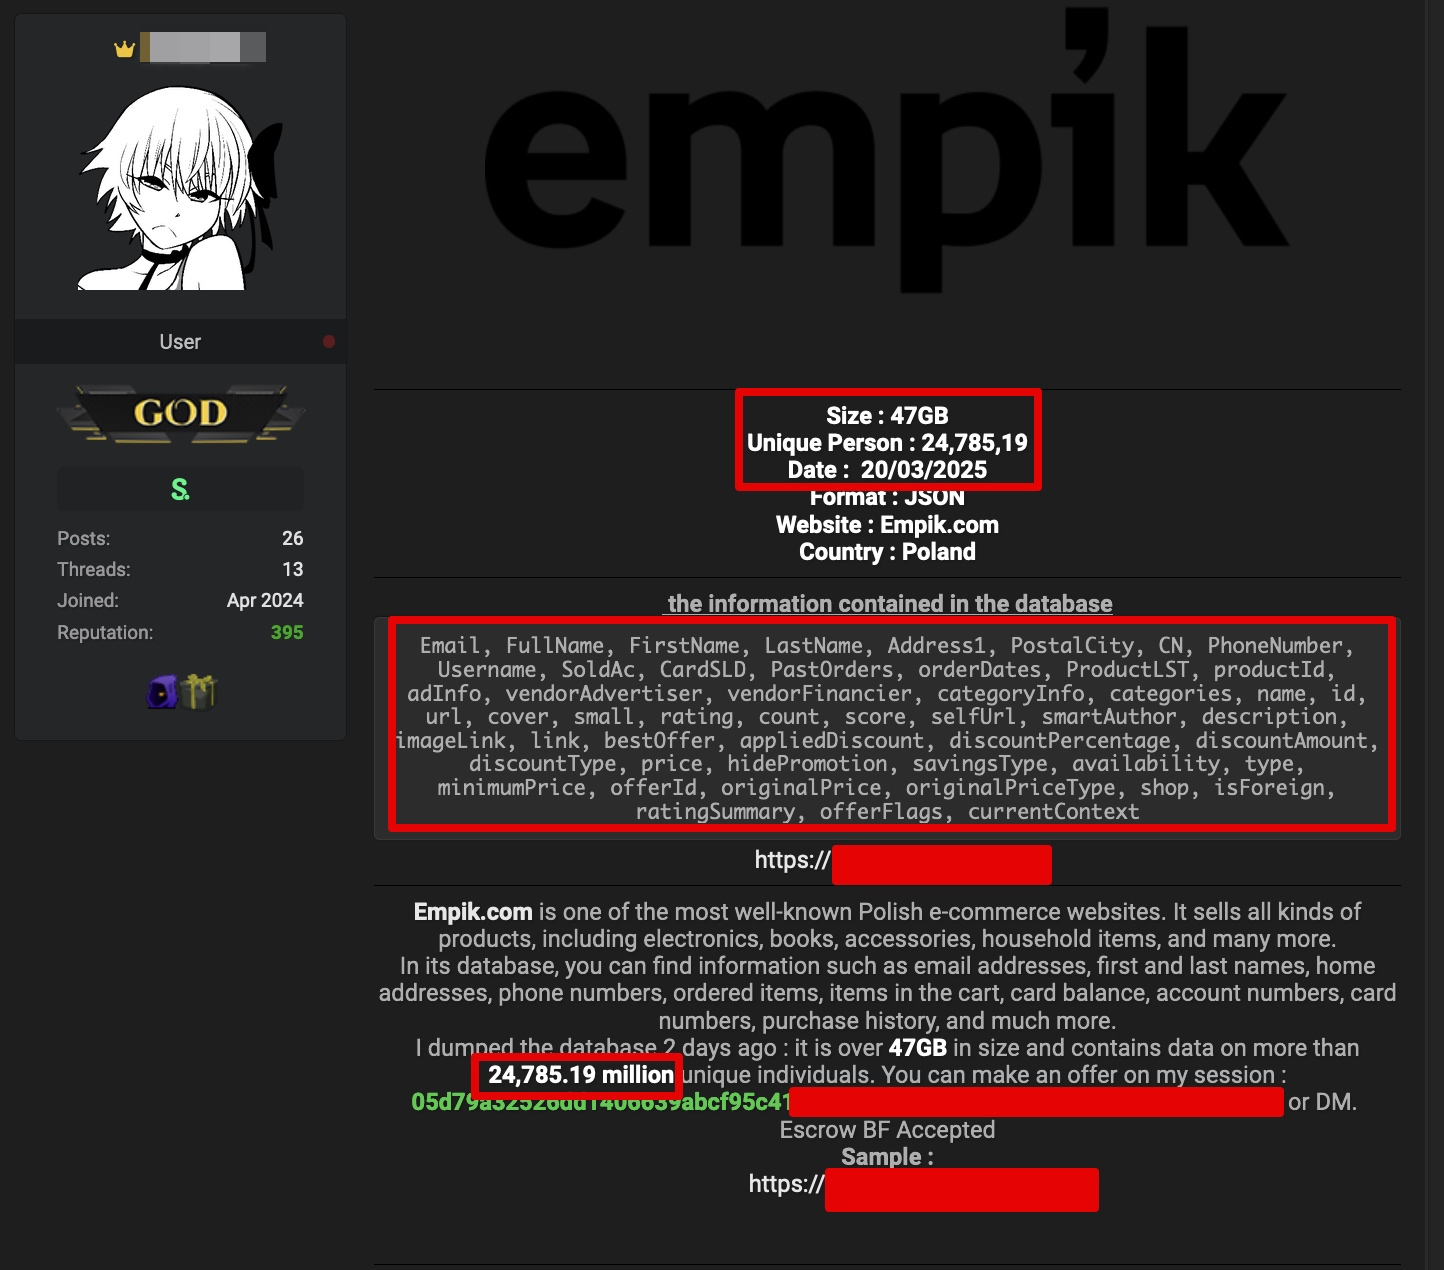
\includegraphics[width=1\textwidth]{images/empik-wyciek.jpg}
\end{columns}
\end{frame}

\begin{frame}{Fałszywe oskarżenie o pedofilię i złodziejstwo}
\begin{columns}[c]
    \column{.55\textwidth}
    \begin{itemize}
      \item Phishing
      \item Kradzież tożsamości
      \item Strach o karierę i reputację
    \end{itemize}
    \column{.45\textwidth}
    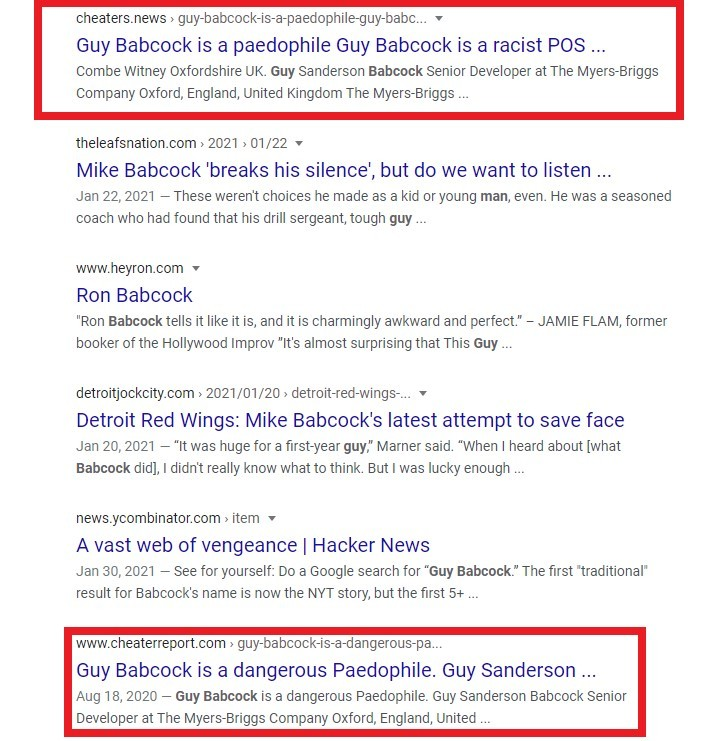
\includegraphics[width=1\textwidth]{images/pedophile.jpg}
\end{columns}
\end{frame}

\begin{frame}{Nękanie i wandalizm}
\begin{columns}[c]
    \column{.65\textwidth}
    \begin{block}{}
      W styczniu 2021 roku senator Mitch McConnell spotkał się z falą krytyki po tym, jak zablokował propozycję zwiększenia kwoty wypłat w ramach rządowej pomocy COVID-19.
    \end{block}
    \column{.35\textwidth}
    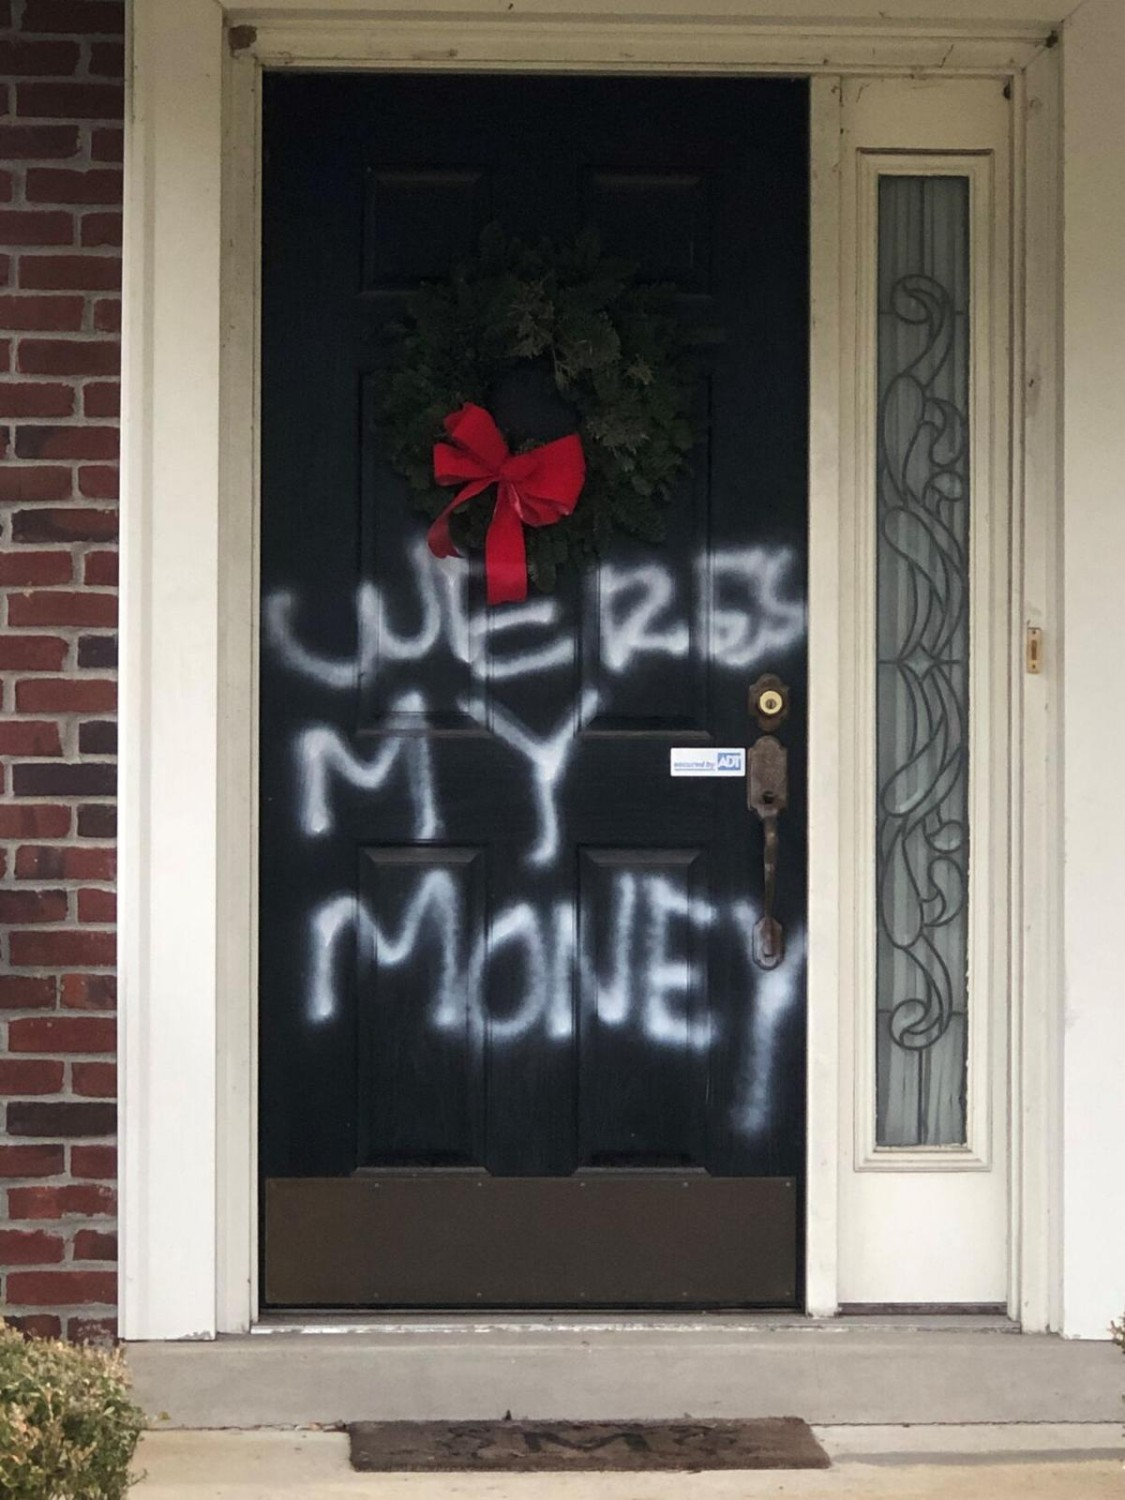
\includegraphics[width=1\textwidth]{images/vandalism.jpg}
\end{columns}
\end{frame}

\begin{frame}{Odpowiedzialność prawna}
    \begin{columns}[c]
      \column{.75\textwidth}
      \begin{block}{}
        Japończyk Hibiki Sato użył zdjęć z mediów społecznościowych i na podstawie refleksów w oczach i Google Street View, by odnaleźć kobietę i ją zaatakować.
      \end{block}
      \column{.25\textwidth}
      
\includegraphics[width=1\textwidth]{images/law.png}
  \end{columns}
\end{frame}
\section{Zalecenia dotyczące prywatności}

\begin{frame}{Świadomość to podstawa}
\begin{alertblock}{Eksperci są zgodni}
Nasza prywatność w sieci zależy przede wszystkim od:
\begin{itemize}
    \item naszej świadomości,
    \item codziennych nawyków,
    \item poziomu ostrożności.
\end{itemize}
\end{alertblock}
\pause
\begin{exampleblock}{Cel: Ochrona przed wyciekiem danych}
Zadbaj o to, co publikujesz. Twoje dane = Twoje bezpieczeństwo.
\end{exampleblock}
\end{frame}

\begin{frame}{Czego nie udostępniać w internecie?}
\begin{itemize}
    \item Adres e-mail, numer telefonu - spam i phishing
    \item Adres domowy, geolokalizacja - ryzyko śledzenia
    \item Zdjęcia dzieci - ochrona prywatności najmłodszych
    \item Kompromitujące zdjęcia - utrata kontroli
    \item Dokumenty osobiste - kradzież tożsamości
    \item Komentarze, skargi - reputacja, odpowiedzialność
    \item Prywatne rozmowy - korzystaj z szyfrowanych komunikatorów \cite{czegoNieUdostepniac}
\end{itemize}
\end{frame}

\section{Jak się chronić?}

\begin{frame}{Zasady cyfrowej higieny}
\begin{columns}[c]
    \column{0.5\textwidth}
    \begin{itemize}
        \item Aktualizuj oprogramowanie
        \item Zabezpiecz sieć Wi-Fi
        \item Używaj silnych haseł
        \item Włącz uwierzytelnianie 2FA
    \end{itemize}
    \column{0.5\textwidth}
    \begin{itemize}
        \item Konfiguruj ustawienia prywatności
        \item Nie klikaj podejrzanych linków
        \item Analizuj usługi „darmowe”
        \item Wyłącz geolokalizację, jeśli niepotrzebna \cite{PROTECTION}
    \end{itemize}
\end{columns}
\end{frame}

\begin{frame}{PESEL - zastrzeżenie to ochrona}
\begin{block}{Co daje zastrzeżenie numeru PESEL?}
\begin{itemize}
    \item Można: zrealizować receptę, przelew, sprawę urzędową
    \item Nie można: wziąć kredytu, otworzyć konta, zmienić umowy
\end{itemize}
\end{block}
\pause
\begin{exampleblock}{Od 1 czerwca 2024 r.}
Banki mają obowiązek sprawdzać zastrzeżenie PESEL przed udzieleniem np. kredytu. \cite{pesel}
\end{exampleblock}
\end{frame}

\begin{frame}{Jak sprawdzić czy wyciekły Twoje dane?}
\begin{itemize}
    \item \href{https://haveibeenpwned.com}{haveibeenpwned.com} - sprawdź, czy Twoje dane wyciekły
    \item \href{https://www.bik.pl/}{BIK} - monitoruj zapytania kredytowe
    \item \href{https://chronpesel.pl/}{chronpesel.pl} - lokalizator wycieku danych
\end{itemize}
\begin{alertblock}{Rada}
Nie czekaj na powiadomienie - samodzielnie monitoruj swoją aktywność.
\end{alertblock}
\end{frame}

\begin{frame}{Co zrobić po wycieku danych?}
\begin{columns}[t]
    \column{0.5\textwidth}
    \textbf{Zmień hasła}
    \begin{itemize}
        \item Minimum 12 znaków
        \item Unikalne dla każdego konta
    \end{itemize}
    \vspace{0.5em}
    \textbf{Zastrzeż dokumenty}
    \begin{itemize}
        \item Dowód, karta płatnicza
        \item W banku lub systemie zastrzegania
    \end{itemize}
    \column{0.5\textwidth}
    \textbf{Zgłoś na policję}
    \begin{itemize}
        \item Gdy doszło do przestępstwa
        \item Zabezpiecz potwierdzenie zgłoszenia \cite{WYCIEK}
    \end{itemize}
\end{columns}
\end{frame}
\begin{frame}{Pytania}
    \begin{center}
        {\huge Pytania?}
    \end{center}
\end{frame}

\setbeamercovered{transparent}
\begin{frame}[allowframebreaks]{Bibliografia}
    \printbibliography
\end{frame}

\begin{frame}{Podziękowania}
    Chcielibyśmy podziękować Panu dr. inż. Janowi Cychnerskiemu za stworzenie 
    i udostępnienie stylu \href{https://github.com/jachoo/pg-beamer}{\emph{pg-beamer}}, 
    co zostało wykorzystane do stworzenia tej prezentacji.\\
    \url{https://github.com/jachoo/pg-beamer}
     
\end{frame}

\begin{frame}{Koniec}
    \begin{center}
        {\huge Dziękujemy za uwagę!}
    \end{center}
\end{frame}

\pglastframe
%wykorzystano ikony z https://www.flaticon.com/packs/network-management-21
\end{document}
